\documentclass[a4paper,fontsize=11pt,report,notitlepage,line_length=38zw,number_of_lines=40,dvipdfmx]{jlreq}
%\usepackage{xltxtra}
%\usepackage{zxjatype}
%\setjamainfont[BoldFont=ipaexm.ttf]{ipaexm.ttf}
%\setjasansfont[BoldFont=ipaexg.ttf]{ipaexg.ttf}

\usepackage{amsmath}
\usepackage{amssymb}
\usepackage{booktabs}
\usepackage{cite}
\usepackage[dvipdfmx]{graphicx}

\title{日本の中古住宅市場における\\スマートコントラクト活用効果の検証}
\author{
学籍番号:57195017 氏名:高橋 宏輝
\\ゼミ名称:ブロックチェーンと分散ファイナンス演習
\\主査:斉藤 賢爾 教授 副査:中里 大輔 教授}

\begin{document}
\date{}
\maketitle
\begin{abstract}
本研究では、日本の中古住宅市場を対象として、住宅の売買取引においてスマートコントラクトをどのように導入できるか検討するとともに、スマートコントラクトの活用により住宅の品質や価格の情報が円滑に共有されることで、住宅の取引価格にどのような影響を及ぼすか検証した。

日本の中古住宅市場は売主と買主の間で住宅の品質などの情報の非対称性が高く、いわゆるレモンの市場であると指摘されている。品質などの情報の非対称性が高い結果、買主は品質が低い可能性を想定し、全ての住宅を安く値付けする。市場の住宅が全て安く値付けされることで、質の良い住宅が市場から淘汰される逆選択が起きている。また、住宅の品質向上に必要なリフォームも、品質情報が共有されない市場では、取引価格の引き上げ効果が期待できないために実施されず、住宅ストック全体の品質向上を妨げている。このような中古住宅市場の問題により、家計が保有する住宅の資産価値は低くなり、家計の活発な消費や投資に繋がらない。

中古住宅市場における情報の非対称性を解消する手法として、住宅取引へのスマートコントラクトの導入を考えた。スマートコントラクトはブロックチェーン上で資産の移転などの処理を行うプログラムである。スマートコントラクトによる資産の移転はブロックチェーン上に改ざん出来ない形で記録され、ブロックチェーンの参加者は誰もがこれらの情報を参照できる。住宅市場へのスマートコントラクトの活用の検討は、契約当事者双方の確実な債務履行や無権利者の排除といったエスクローとしての検討が中心であった。しかし、情報の非対称性が高い住宅市場においては、エスクローとしての活用に加えて、住宅取引情報のデータベースとしての活用の効果も大きい。ただし、価格などの住宅取引情報は、取引参加者にとって公開したくない情報である可能性が高いことから、データベースとしての活用にあたっては、参照される情報に一定の匿名性が必要となる。本研究では、これらの点を考慮したスマートコントラクトの仕様を検討した。

スマートコントラクトの活用によって、住宅の品質や過去の取引価格などの情報が全ての参加者から参照可能となった場合、住宅取引にどのような影響が発生するか検証するため、住宅取引を単純化したゲームによるマルチエージェントシミュレーションを行った。その結果、品質の情報が買主から参照可能になる事によって、市場全体として見た場合の売主の利得は向上し、成約率も改善することが確認できた。

日本の住宅市場では、人口が減少に転じ、800万戸を超える住宅が空き家になっているにもかかわらず、年間90万戸の住宅が新たに供給されている。このような状況は、中古住宅市場の情報の非対称性により質の良い中古住宅が市場に供給さず、市場が活性化しないことが要因となり発生していると考えられる。スマートコントラクトでの住宅取引により情報の非対称性が解消され、住宅が品質に応じて適正に値付けされる市場を形成できれば、質の良い中古住宅の市場供給も増え、取引量も増えると考えられる。

\end{abstract}

\newpage
\tableofcontents

\newpage
\chapter{序論}
\section{本研究の動機}
日本の住宅市場は新築住宅に偏重しており、中古住宅の流通量は少ない。2015年の国土交通白書によると日本の住宅取引全体に占める中古住宅取引の割合は14.7\%であり、アメリカ(同89.3\%)、イギリスの(同88.0\%)、フランス(同68.4\%)と比較して大幅に低い水準となっている\cite{hakusho}。一方で、総務省の住宅・土地統計調査によると、日本の住宅総数は、2018年の段階で総世帯数に対して約879万戸超過している。居住者のいない住宅は都市部でも顕著であり、首都圏の一都三県における居住者のいない住宅戸数は200万戸を超えている。しかし、中古住宅市場の流通量は少なく、これらの居住者がいない住宅ストックの活用が進んでいない。このため、日本の住宅は新築から25年程度で建物の価値が半分になると指摘されている(吉田 2016)\cite{yoshida2016}。
また、住宅が平均して建築後何年で取り壊されているかを調査した滅失住宅の平均築後年数は、アメリカが66.6年、イギリスが80.6年であるのに対し、日本は32.1年であり、より短い期間で住宅が取り壊されていることがわかる\cite{kizonjutaku}。

次に日本の家計の資産構成を見ると、他国よりも資産としての寿命の短い住宅が資産構成において大きな割合を占めている。日本の家計が保有する住宅・宅地資産の総額は1,000兆円を超えると言われており、家計が保有する現金・預金等の総額940兆円を上回る。しかし、日本において住宅の建物部分の価値は短い期間で減少してしまうため、国内でこれまでに行われた住宅投資の累計が約890兆円にのぼるのに対し、その現在評価額は投資額累計を500兆円以上下回る約350兆円程度であると指摘されている\cite{roundtable}。一方で、アメリカでは減価償却以上に修繕やリフォームが行われる事により住宅資産額が住宅投資額累計を上回る状況にある。このことから、アメリカでは住宅が資産として活用されているが、日本では耐久諸費材として消費されているとの指摘がされている(小島 2013)\cite{kojima2013}。
中古住宅の評価が改善され、家計が保有する住宅資産の価値が向上すれば、住宅を資金化した場合の金融資産の増大に繋がり、それが投資や消費に回ることで日本経済に好循環をもたらすことが期待できる。

日本で中古住宅の活用が進まない背景には、日本人が過度に新築を好むといった心情の問題だけではなく、消費者が中古住宅の品質や価格に不安や懸念を抱いていることも影響している。国土交通省の住宅市場動向調査において、新築の注文住宅、分譲住宅、分譲マンションの購入者に、なぜ中古住宅を購入しなかったか、理由を聞いた結果が表\ref{doukou}の通りであり、住宅の品質や瑕疵の存在を懸念して中古住宅を購入しなかった層が多数存在していることが分かる。山崎(2014)\cite{yamasaki2014}が指摘する通り、日本の中古住宅市場は、買主が中古住宅についての情報を十分に得ることができず、売主と買主の間で大きな情報の非対称性が存在する「レモンの市場」となっている。買主は住宅の品質情報を持たないため、品質が低い可能性を考慮して全ての住宅について購入価格を引き下げる。全ての住宅の購入価格が引き下げられる結果、質の良い住宅が市場から淘汰される逆選択が起こる。このことが日本の中古住宅市場が拡大しない大きな要因であると考えられる。

\begin{table}[!h]
\begin{center}
\caption{中古住宅を購入しなかった理由(複数回答)}
\label{doukou}
\begin{tabular}{|l|r|r|r|}
\hline
&
\begin{tabular}{c}
注文住宅\\取得世帯
\end{tabular}
&
\begin{tabular}{c}
分譲戸建住宅\\取得世帯
\end{tabular}
&
\begin{tabular}{c}
分譲マンション\\取得世帯
\end{tabular}\\ \hline

新築の方が気持ち良いから& 61.5\% & 66.8\% & 60.6\% \\
リフォーム費用などで割高になる& 31.5\% & 31.9\% & 30.9\% \\
隠れた不具合が心配だった& 26.9\% & 26.7\% & 24.5\% \\
耐震性や断熱性など品質が低そう& 31.3\% & 17.9\% & 20.7\% \\
給排水管などの設備の老朽化が懸念& 19.0\% & 17.0\% & 29.8\% \\
間取りや台所等の設備や広さが不満& 18.0\% & 13.1\% & 11.2\% \\
価格が妥当なのか判断できない& 6.6\% & 11.9\% & 14.4\% \\ \hline
\end{tabular}
\begin{tabular}{r}
出所:国土交通省「平成30年 住宅動向調査」より筆者作成
\end{tabular}
\end{center}
\end{table}


中古住宅市場が拡大しない結果、ライフステージの変化に応じて住宅を売却し、住み替えを行うという動因が所有者に働きにくい。そのため、日本では建築主の趣味に合わせた間取りやデザインを優先する注文住宅の比率が高くなっている。日本の新築住宅に占める注文住宅の割合は7割程度、建売の分譲住宅は3割程度であるが、アメリカではこの比率が逆転しており建売の分譲住宅の方が一般的である。さらに、所有期間中のメンテナンスも、日本では必要最小限が行われるのみであり、建物の価値を維持、向上する観点からのメンテナンスが行われていない。情報の非対称性により中古住宅市場が活性化しないことで、質の良い中古住宅の市場供給が妨げられ、さらに買主が中古住宅を敬遠する悪循環が発生している。

\section{本研究の貢献}
中古住宅市場が抱えるこれらの問題を解消するためには、市場の全ての参加者が住宅の品質や価格について、取引実績を参照でき、取引対象の住宅の品質情報を正しく把握できることが必要であると考えられる。日本の既存住宅市場における情報開示量が成約価格や成約率、売り出し価格に与える影響について、藤澤(2016)\cite{fujisawa2016}は住宅の品質情報がわかりやすく全開示情報となれば良質な維持管理へのインセンティブを与えると指摘している。現在でも取引実績の情報を提供する取り組みや品質情報を把握するための制度は存在するが、様々な理由から普及しているとは言い難い。本研究では住宅市場が持つ情報の非対称性の問題を解消する方法として、スマートコントラクトの住宅取引への導入を検討する。スマートコントラクトは、ブロックチェーン上で資産の移転を行うプログラムである。スマートコントラクトの基盤となるブロックチェーンは、特定のルールによって検証された情報が納められたブロックの繋がりであり、ブロックに納められた情報が全ての参加者から参照可能であり、その情報は現実的に改ざんが不可能であるという特徴がある。このため、スマートコントラクトを活用して住宅の品質情報の登録や売買取引を行えば、それらの情報が、修正や改ざんが加えられず、誰にでも参照可能な形で記録されることになり、情報の非対称性の問題に寄与すると考えられる。

\section{本論文の構成}
本論文では、第2章において日本の中古住宅市場の特徴をより詳細に確認し、住宅の価格決定に関する先行研究を整理するとともに、スマートコントラクトの概要を整理する。第3章では住宅取引へのスマートコントラクト導入の検討について述べる。第4章ではスマートコントラクトが住宅取引にもたらす影響を検討するため、マルチエージェントシミュレーションによる検証の方法を述べる、第5章でシミュレーションの評価を行う。第6章で関連研究との比較を行い、第7章は結論となる。


\chapter{背景}
\section{日本の住宅市場}
\subsection{日本の住宅市場の概要}
日本の総住宅数と総世帯数の関係を見ると、1968年の調査で総住宅数が総世帯数を上回り、直近では総世帯数の1.16倍の住宅が存在している。2018年10月1日時点で日本国内には約6240万戸の住宅があり、この内879万戸には誰も居住していない。人が居住していない住宅のうち、賃貸用の住宅や売却用の住宅を除いた「空き家」は348万戸存在している\cite{tochitokei}。人が居住している住宅の所有関係を見ると、約6割が持ち家で約4割が借家となっている。総世帯数に対して総住宅数が大幅に超過している状況でも、日本では毎年90万戸程度の住宅が新たに供給されている\cite{kenchikuchakkou}。11万戸程度の住宅が取り壊されているが、新規供給数が多いため、総住宅数も空き家も年々増加している。前述の通り、日本の住宅は取り壊しまでの期間が短く、住宅が頻繁に建て替えられる状況については、CO2の排出など環境面の負荷も指摘されている(The Guardian 2014)\cite{guardian}。

日本国内の中古住宅の取引は、戸建て住宅が年間18万件、マンションが19万件程度行われている。取引主体別の件数を見ると、売主、買主がともに個人同士で行われてる取引が、戸建て住宅で53\%、マンションで45\%であり、最も多い\cite{fudosantorihiki}。住宅をはじめとした不動産の取引は、売主と買主の仲介を行う宅地建物取引業者を介して行われることが一般的であり、売主、買主がともに個人同士の取引においても同様である。宅地建物取引業者が不動産情報の交換を行う仕組みとして不動産流通機構の「レインズ(REINS:Real Estate Information Network System)」がある。これは、不動産流通機構の会員である宅地建物取引業者がアクセスできるシステムであり、住宅の売却や購入を希望する個人は直接アクセスすることができない。宅地建物取引業者は、売却や購入の仲介の依頼を受けた情報を、必ずしも全てレインズに登録する必要はない。また、レインズに登録した物件の取引が成立した場合も、その情報がレインズに登録されない場合もある\cite{fudosanjoho}。住宅以外も含めたレインズへの売却物件の新規登録件数は、2019年が169万件であり、成約報告件数は18万件である\cite{shiteiryutsu}。

\subsection{日本の住宅行政}
日本の住宅行政の方向性を示しているのが2016年に見直しが行われた住生活基本計画である\cite{juseikatsu}。この計画では、住生活をめぐる今後10年の課題として、少子高齢化と人口減少、これに伴う空き家の増加に加えて、「リフォーム・既存住宅流通等の住宅ストック活用型市場への転換の遅れ」が指摘されている。そのうえで、「購入した住宅の維持管理やリフォームの適切な実施により、住宅の価値が低下せず、良質で魅力的な既存住宅として市場で評価され、流通することにより、資産として次の世代に承継されていく新たな流れ(新たな住宅循環システム)を創出」することを目標の一つとして挙げている。この目標を達成するため、以下の5つの基本的な施策を設定している。
\begin{itemize}
\item 建物状況調査(インスペクション)、住宅瑕疵保険等を活用した品質確保
\item 建物状況調査(インスペクション)における人材育成や非破壊検査技術の活用等による検査の質の確保・向上
\item 住宅性能表示、住宅履歴情報等を活用した消費者への情報提供の充実
\item 内装・外装のリフォームやデザインなど、消費者が住みたい・買いたいと思う既存住宅の魅力の向上
\item 既存住宅の価値向上を反映した評価方法の普及・定着
\end{itemize}

\subsection{建物状況調査と住宅瑕疵保険}
住生活基本計画の施策として挙げられている建物状況調査は、中古住宅の基礎や外壁のひび割れや雨漏りといった劣化・不具合の状況を調査するもので、国の登録を受けた技術者が実施する。2018年に行われた宅地建物取引業法の改正によって、売買の仲介をする宅地建物取引業者は、中古住宅の売買時に建物状況調査の制度概要等の説明を行うことが求められるようになった。また、売買対象の建物について、過去1年以内に建物状況調査が実施されている場合には、売買にあたって作成される重要事項説明書において劣化事象等の有無を説明することとされている\cite{takuchitatemono}。

新築住宅の売買において売主は、主要な構造部分の瑕疵について10年間の瑕疵担保責任を負うことが法律上定められているが、中古住宅の売買においてはそのような制度がない。そのため、中古住宅の売買において買主を保護する必要が指摘されていた。既存住宅売買瑕疵保険は、中古住宅を売買する際に加入することができる保険で、住宅の主要な構造部分や屋根などに瑕疵が発見された場合に補修費用等が支払われる保険である。この保険は、2007年に施行された「特定住宅瑕疵担保責任の履行の確保等に関する法律(住宅瑕疵担保履行法)」に基づいて創設されたもので、国土交通大臣が指定した住宅瑕疵担保責任保険法人という住宅専門の保険会社が保険契約を締結することができる。現在は5つの法人が業務を行なっている。

建物状況調査も既存住宅瑕疵保険も、中古住宅の売買にあたって利用が義務付けられているものではなく、活用は進んでいない。2018年の建物状況調査の実施件数は6,736件\cite{questionnaire}であり、同年の中古住宅売買の4\%程度でしか利用されていない。

\subsection{住宅性能表示制度と住宅履歴情報の提供}
住宅性能表示制度は、2000年に施行された「住宅の品質確保の促進等に関する法律」に基づく制度で、戸建て住宅とマンション等の共同住宅について、新築住宅と既存住宅の双方で活用することができる制度である。既存住宅の性能表示では、地震などへの耐久性や省エネルギー性、防犯対策、配管等の維持更新のし易さ等の性能項目と現況における劣化の状況について、第三者機関による評価が行われる。住宅性能表示制度は、新築住宅については、2019年時点で新設住宅着工件数の27.7\%に当たる245,156戸が評価書の交付を受けている。一方で、既存住宅については、2019年の評価書交付実績は400戸であり、利用が広がっていない\cite{jutakuseino}。藤澤他(2004)\cite{fujisawa2004}は、住宅性能表示制度の問題点として、性能評価書の取得に手間がかかることで、買主が性能評価書に基づいた比較購買をし難い点を指摘している。


\subsection{リフォーム}
質の良い住宅ストックの形成にはリフォームが欠かせない。しかしながら、日本の住宅市場においてリフォームの実施率は高くない。これは、リフォームを行っても住宅価格に反映されないため、住宅の所有者にリフォームのインセンティブが働かないと考えられる。原野他(2012)\cite{harano2013}は、住宅の所有者によるリフォームは、大規模なリフォームであっても取引価格の引き上げ効果は観察できず、小規模なリフォームでは不動産業者によるリフォームでも取引価格の引き上げ効果が確認できないと指摘している。そして、この事態の改善には、中古住宅を取引する時点で住宅の品質を正確に把握することが重要であり、建物状況調査により品質に関する情報の非対称性を解消することが可能と考察している。


\subsection{取得可能な不動産の情報}
住宅の売買を行う際に参照できる情報として、国土交通省が提供している土地総合情報システム\footnote{https://www.land.mlit.go.jp/webland}における不動産取引価格情報がある。これは、不動産の取引当事者を対象としたアンケート調査の結果を物件等を特定できないように加工して公表しているもので、土地取引だけでなく中古マンションや戸建て住宅についても調査・公表が行われている。この情報は調査対象の物件が所在する地域の不動産価格について、ある程度の参考にはなるものの、調査対象の物件の品質などの個別情報は提供されていないこと、情報がアンケート調査によるものであることなど、活用に限界がある。
不動産仲介を行う宅地建物取引業者が利用できるシステムとしては前述のレインズがあるが、消費者は利用できない。藤澤(2016)\cite{fujisawa2016}
は、「良質なストック住宅を形成するためには,良質であることを売主がアピールできることと,買主が質を認識できることが必要である」と指摘しているが、中古住宅の主要な売主、買主である個人が利用可能な情報源は限られており、情報の非対称性が生まれる背景となっている。


\section{住宅価格についての先行研究}
\subsection{サーチ理論}
住宅市場は中央集権的な取引市場が存在せず、取引は局所的に、売主と買主の相対取引(Over The Counter)で行われることが一般的である。このような局所的、分権的取引のミクロ構造をモデル化しようとする取り組みとしてサーチ理論がある。サーチ理論の一つである両方向サーチ・モデルでは、売主、買主ともに取引相手を探し、出会った場合に取引を前提として価格の交渉を行う状況を分析対象とし、局所的に無数の取引が繰り返される中で経済全体としては均衡しているという状況を描写することができる(今井他 2007)\cite{imai2007}。両方向サーチ・モデルは市場参加者の出会い方によってランダム・サーチモデルやディレクテッド・サーチモデルなどがある。ランダム・サーチでは、売主と買主は偶然出会った相手と価格交渉を行う。一方でディレクテッド・サーチでは、参加者は相手側の提示価格を見て交渉に臨むことができる。ディレクテッド・サーチでは、出会い確率や取引確率が価格に応じて変化する状況を説明することができる。Wheaton(1990)\cite{wheaton1990}はランダム・サーチモデルを住宅市場に導入し、買主が売主でもある住宅市場の特性から、価格と空室の関係を分析した。ランダム・サーチモデルにおいては、住宅価格と市場規模には正の相関があり、各種の摩擦が住宅市場の明確さに影響しているとされる(Han and Strange 2015)\cite{han2015}。
Diaz and Jerez(2013)\cite{diaz2013}は、売主があらかじめ価格を設定して、買主がそれを見て購入を申し込むディレクテッド・サーチモデルを導入し、住宅市場の流動性が高いときには住宅価格も高くなるモデルを提唱した。ディレクテッド・サーチは市場の摩擦を表現できるモデルであるが、住宅市場への導入においては、仲介者の存在を考慮する必要がある。彼らは売主でも買主でもあり、売り出し価格の決定に複雑な影響を与えている(Han and Strange  2015)\cite{han2015}。

\subsection{相対取引における住宅価格の決定}
相対取引では、取引相手を探す「探索」と取引相手との「交渉」による摩擦が取引の流動性を減じるため、その分だけ取引価格から減額される。これを非流動性ディスカウントと呼ぶ。住宅市場の参加者を住宅の所有の有無と住宅の所有意向の高低で4つのグループに分けた場合、全ての参加者が、住宅の所有意向が高く住宅を所有しているグループと住宅の所有意向が低く住宅を所有していないグループのいずれかに属していれば均衡となり取引は発生しない。その状態から、転勤や転職など住宅価格とは無関係の事象によって参加者の住宅所有意向が変動すると、住宅の売り出しや購入に向けた探索が始まる。
Duffie et al(2006)\cite{duffie2007}は、取引相手を探すのが難しい場合、売買交渉における売主の交渉力が弱い場合、市場における資産の適格な所有者のシェアが小さい場合、リスク回避の需要が大きい場合に非流動性ディスカウントが大きくなると指摘した。住宅の価格水準は実際の取引価格によって測定されるが、住宅は売買される機会が少ないため、住宅全体の価格水準が少ない取引実績を基準として測定されている。そのため、少数の楽観的な投資家の存在により、住宅価格全体が引き上げられる。Piazzesi and Schneider(2009)\cite{piazzesi2009}は、住宅市場における楽観的な参加者が住宅価格に与える影響を以下の式で与えた。

%住宅の品質を新築時に決まるものと、所有期間における維持管理によって決まるものに分類し、売主は住宅を売却する段階で品質を変更することはできず、品質を所与として価格設定を行うものとする。売主は住宅を所有するもの中から$\lambda_{d}$の確率で発生するとする。藤澤(2016)では、売主と買主はそれぞれ同数として、売主、買主の探索の摩擦を考慮していない。しかし、現実の住宅取引においては、売主と買主の数は等しいとは限らない。Duffie(2007)は売主の数が買主よりも少ない場合、取引価格は減少すると指摘している。そこで本研究では、住宅の所有者のうち、一定の確率で住宅を所有する意思が低下し、

\begin{equation}
P=\dfrac{v}{r}-\dfrac{\eta}{r+\eta+m}\dfrac{v+c}{v}
\end{equation}

ここで、左辺$P$は住宅価格、$r$は割引率、$v$は住宅環境を得るためのコスト(家賃)、$\eta$は住宅の所有者に住宅を売却する事情(転勤や転職など)が発生する確率、$m$は売主と買主が出会う率、$c$は住宅取引の費用である。
右辺の第一項は家賃収入(配当)の割引現在価値、第二項は非流動性ディスカウントを表している。売却する事情が発生しても、通常はすぐには売却できず、売却できるまでの間家賃を得ることができないが、出会う率が無限大であれば第二項はゼロになり、非流動性ディスカウントは消失する。

\subsection{住宅サービスのコスト}
住宅の保有コストは、住宅投資の資本コストに相当するものであり、住宅の価格、利子率、減価償却率、保有税率、維持管理費、住宅価格の変化率に依存している。
また、住宅サービスの利用コストから整理すると、住宅の価格を$P$、減価償却率を$\delta$、維持管理費を$\mu$、保有税率を$\tau$、住宅ローンの利子率を$i$、住宅価格の上昇率を$\pi_H$とすると、保有コストを$C$は以下の式で表すことができる(川口 2013)\cite{kawaguchi2013}。

\begin{equation}
C=P\times(\delta+\mu+\tau+i-\pi_H)
\end{equation}

摩擦のない市場では資本の限界収益率がユーザーコストと等しくなるときが最適な投資となるため、住宅市場における最適な投資が行われている世界では住宅の賃料と保有コストは等しくなる。賃料を$R$とした場合、$R=C$となるように住宅の供給が決まると考えられる。しかし、実証分析では賃料と保有コストの間に乖離が確認されている(Garner and Verbrugge 2009)\cite{garner2009}。賃料と保有コストの乖離についてChinloy et al(2020)\cite{chinloy2020}は、賃料が限界費用コストに加えて住宅ローンやインフレのショックを回避するためのプレミアムを含んでいると指摘している。

\section{スマートコントラクト}
\subsection{ブロックチェーン}
ブロックチェーンは、あるルールによって検証された情報が納められたブロックの繋がりであり、一度ブロックに納められた情報はブロック同士の繋がりを維持したまま変更することができないため、現実的に改ざんが不可能となる。ブロックチェーンには全ての情報を一元管理する存在がなく、参加者(ノード)がそれぞれに同じ情報を保有しあっており、参加者は全てのブロックの情報を参照できるようになっている。ブロックチェーンの信頼性は、情報をブロックに納める際のコストで担保されるが、このコストは大きな計算能力の浪費という形態をとる。このコストを支払う参加者をマイナーと呼び、マイナーは参加しているブロックチェーンのネイティブ通貨で報酬を受け取り情報の検証作業を行う。斉藤(2017)\cite{saito2017}はブロックチェーンの機能の階層構造を「正当性の保証」、「存在性の証明」、「唯一性の合意」、「ルールの記述・執行」で整理している。正当性の保証は、ブロックチェーン上の情報がルールに基づいて改ざん不可能な形で記述されており、過去の履歴と矛盾しないことを保証する機能である。この機能は、正当な権限を持つ参加者か否かをデジタル署名などにより検証し、正当な参加者による情報の投入も保証している。存在性の証明は、過去に遡って情報を抹消したり捏造できない仕組みである。唯一性の合意は、情報の履歴やブロックの繋がりが全ての参加者からみて単一であると合意するための機能である。ルールの記述・執行は、正当性を確認するためのルールや自動処理の設計、実行を行う機能であり、この機能により記述されたルールがスマートコントラクトである。

\subsection{スマートコントラクト}
スマートコントラクトは、ブロックチェーン上で資産の移転などの処理を行うプログラムであり、法的な契約ではない。従来の紙や電子契約においては、契約の条件が満たされているかの判断は自動では行われず、各契約当事者が確認を行う必要があった。スマートコントラクトでは、契約の条件が満たされたかの確認はプログラムが行い、契約内容の執行はブロックチェーン上の価値の移転によって自動的に行うことができる。スマートコントラクトで実行された内容はブロックチェーン上に改ざんできない形で記載されるため、取り消すことができない。これはCode is lawとよく言われる概念であり、スマートコントラクトにおいては、ブロックチェーン上に書かれたプログラムが、契約書であり、裁判所でもあることになる\cite{nagasawa2013}。
スマートコントラクトが実行されるブロックチェーンネットワークには、パブリックとプライベートの区別がある。パブリックブロックチェーンは誰でも読み込み、書き込むことができる。プライベートブロックチェーンではユーザー毎に異なる権限設定を行える。イーサリアム、Bitcoinはパブリックブロックチェーンであり、プライベートブロックチェーンとしてはHyperledger Fabricなどがある。

\subsection{イーサリアムブロックチェーンとスマートコントラクト}
イーサリアムブロックチェーンは、スマートコントラクトを実装する基盤として多く用いられている。イーサリアムブロックチェーンでは、外部所有アカウント(EOA)とコントラクトアカウントの2種類のアカウントがあり、外部所有アカウントはブロックチェーンの参加者によって、参加者のために作成されたアカウントで秘密鍵を持っている。コントラクトアカウントは秘密鍵を持たず、スマートコントラクトコードによって制御されるアカウントである。これらのアカウントはアドレスやネイティブ通貨であるEtherの残高などの情報を持っている。トランザクションは、外部所有アカウントから発信される署名付きのメッセージで、イーサリアムの状態の変更やスマートコントラクトの実行ができる。スマートコントラクトを実行するためのトランザクションを発信できるのは外部所有アカウントのみだが、スマートコントラクトにより制御されたコントラクトアカウントは、他のコントラクトアカウントを呼び出すことができる。イーサリアムブロックチェーンにおいてスマートコントラクトを実行する場合、ガスと呼ばれる費用がかかり、計算能力を提供するマイナーへの報酬となる。通常、コントラクトを実行する際には、使用されるガスの上限であるガスリミットを設定する。費用の総額は、プログラムの実行にあたって使用された計算能力とストレージの使用量に基づくガス量に、Etherを単位とするガスの単価を乗じて算出される。ガスは、トランザクションの送信者によって負担され、トランザクションの送信者はガスの単価を指定する。マイナーは、未処理のトランザクションの中から単価の高いトランザクションを選んで処理できるため、高いガスの単価を提示すれば、より早くそのトランザクションは処理される(Antonopoulos and Wood 2019)\cite{antonopoulos2019}。

\subsection{住宅・不動産分野における活用事例}
スマートコントラクトの概念は、イーサリアムなどのブロックチェーン基盤が導入されて以降、顕著に発展しているが、現時点では「デジタルに表現される資産をあらかじめ定められたルールに従って自動的に移転させることにすぎず、また、そのことすら実現上の課題が多い」(斉藤2017)\cite{saito2017}との指摘がされている。スマートコントラクトの住宅取引への活用事例としては、アメリカのPROPY\footnote{https://propy.com}がある。同社は不動産の売買取引において、売主と買主を取り持つ第三者として、売主から権利証書、買主から売買代金を預かり、行政の登記手続きが終了するまでの間、ブロックチェーン上に取引の情報を記録し、登記手続きが完了すると権利証書と売買代金の移転を行うというサービスをオンライン上で提供している。同じくアメリカのRentberry\footnote{https://rentberry.com}は、アメリカおよびヨーロッパの都市部において賃貸住宅の仲介サービスを提供しており、入居者はオンライン上で全ての契約手続きを完了させることができる。さらに、Rentberryでは、敷金の支払いが困難な入居者が、第三者から敷金を借り入れできるP2Pレンディングサービスも提供している。

日本国内での不動産分野におけるスマートコントラクト活用事例としては、株式会社GA technologiesによる不動産賃貸契約へのスマートコントラクト導入の取り組みがある\footnote{https://www.ga-tech.co.jp/news/1600/}。この取り組みは、IBMがHyperledger Fabricを基盤として提供しているIBM Blockchain Platform上で開発を行うとの発表されていた。しかし、その後実用化したとの発表はない。

\chapter{住宅市場へのスマートコントラクトの導入}
\section{解くべき問題}
中古住宅市場における問題は、売主と買主の間で住宅の品質に関する情報が共有されておらず、適切な値付けが行われないことである。買主としては住宅の品質が分からない以上、品質が低い場合にも損をしないような値段づけを行うことになる。これに対して、売主、買主以外の第三者が、取引対象の住宅について、その品質を調査し、検証を行い、その情報をブロックチェーン上に記録することを検討した。これにより、買主は住宅の品質を確認できるようになり、ブロックチェーン上の他の売買事例を参考にして、購入検討している住宅をより適正に値付けできる。現状で利用可能なアンケート調査や仲介業者の自己申告のように、修正や改ざんの余地がある方法で収集された情報では、情報全体の信頼性が下がる。そのため、実際の建物状況調査の結果や取引価格などの情報が、修正や改ざんがされない形で収集されることが重要である。この観点で、スマートコントラクトによって住宅取引を行い、その住宅取引の情報がブロックチェーン上に記録され、取引当事者以外のブロックチェーンの参加者が誰でも実際の取引情報を参照できることが重要である。一方で、住宅の品質や過去の取引価格は、住宅の所有者にとって、他者に知られたくない情報である可能性が高い。個別の住宅の品質情報や価格情報を市場に提供すればするほど、市場における情報の非対称性は是正され、品質の不透明性によるディスカントは解消されると考えられるが、プライバシーが侵害されるのであれば、それらの情報を提供するインセンティブが働きにくい。日本の中古住宅市場が抱える課題の解決には、情報の匿名性を確保した上で、価格や品質の情報に誰もがアクセスできる仕組みを作ることが必要であり、スマートコントラクトによる住宅取引は有効な解決策になり得る。

\section{住宅取引の関与者}
本研究ではイーサリアムブロックチェーンを基盤とするスマートコントラクトでの住宅取引を検討した。このスマートコントラクトの関与者は売主、買主に加えて、住宅の品質を調査するインスペクター、インスペクターが評価した品質情報を検証し、予期しない瑕疵が発生した場合に修理費用などを保証する保険会社であり、これらが外部所有アカウントである。コントラクトアカウントとしては住宅アセット、保険契約、住宅取引契約がある。それぞれのアカウントの定義及び保有する情報は以下の通りである。
\begin{itemize}
	\item 売主
    \par 住宅アセットに所有者として登録されている外部所有アカウント。住宅取引契約の実施にあたりトランザクションを作成し送信することができる。
    \item 買主
    \par 住宅取引契約で売主の相手方となる外部所有アカウント。購入代金としてEtherを所有している。住宅取引契約の実施にあたりトランザクションを作成し送信することができる。
    \item インスペクター
    \par 建物状況調査の実施資格を持つ外部所有アカウント。住宅アセットに住宅性能表示の情報を登録できる。
    \item 保険会社
    \par 住宅瑕疵担保責任保険法人である外部所有アカウント。インスペクターが行った住宅性能表示を検証する。保険契約における保険会社であり、予期しない瑕疵が発生した場合には修理費用などを支払う。
	\item 住宅アセット	
	\par 土地及び土地に付属する建物の所有権をデジタル資産として表現したコントラクトアカウント。他の住宅アセットと識別するための住所、面積、取引価格の履歴、所有者のアドレス、住宅性能表示、保険契約のアドレスの情報を持つ。所有者のアドレス、住所以外の情報は第三者から参照可能となっている。
	\item 保険契約
    \par 保険契約を行うコントラクトアカウント。売主または買主のトランザクションで開始される。インスペクターに住宅性能表示の実施を指示し、保険会社には住宅性能表示の検証を指示する。
    \item 住宅取引契約
    \par 住宅アセットの所有者変更を行うコントラクトアカウント。売主または買主のトランザクションで開始される。売主からの所有権移転トランザクションと買主の送金トランザクションが揃った場合に住宅アセットに所有者移転のトランザクションを送る。
\end{itemize}

\section{取引情報の検索}
転職や結婚などの事情により、住宅の売却または購入を行う場合、人々はそれぞれに自身が所有する住宅がいくらで売れるか、自身が購入を希望する住宅がいくらで買えるか相場を調べる。スマートコントラクトを用いた住宅取引では、住宅アセットのコントラクトアカウントがそれぞれに住宅性能表示や過去の取引価格の情報を保有している。売主は自身が所有する住宅の住所で、買主は購入を希望する住所で検索を行い、それぞれに品質と価格の相場情報を得ることができる(図\ref{search})。ここで、住所情報の取り扱いに注意する必要がある。住所情報自体が参照可能になると個々の住宅を特定することができる。一般に住宅の所有者にとって、自身が所有する住宅の取得価格や品質は他者に知られたくない情報だと考えられる。そのため、取引情報の検索を行った場合に返される値は品質情報と価格情報のみとし、それらが住所情報と紐づいた状態で参照できない設計とする事が、参加者のプライバシー保護の観点から重要である。住所情報自体が参照できない設計であっても、検索条件に合致する住宅アセットの数が極端に少なかった場合、実質的に住宅の特定が可能となる場合がある。検索結果が極端に少ない状況を回避するため、図\ref{flow}のような処理を行い、少なくとも20件以上の検索結果を出力させる処理を行う。

\begin{figure}
 \centering
 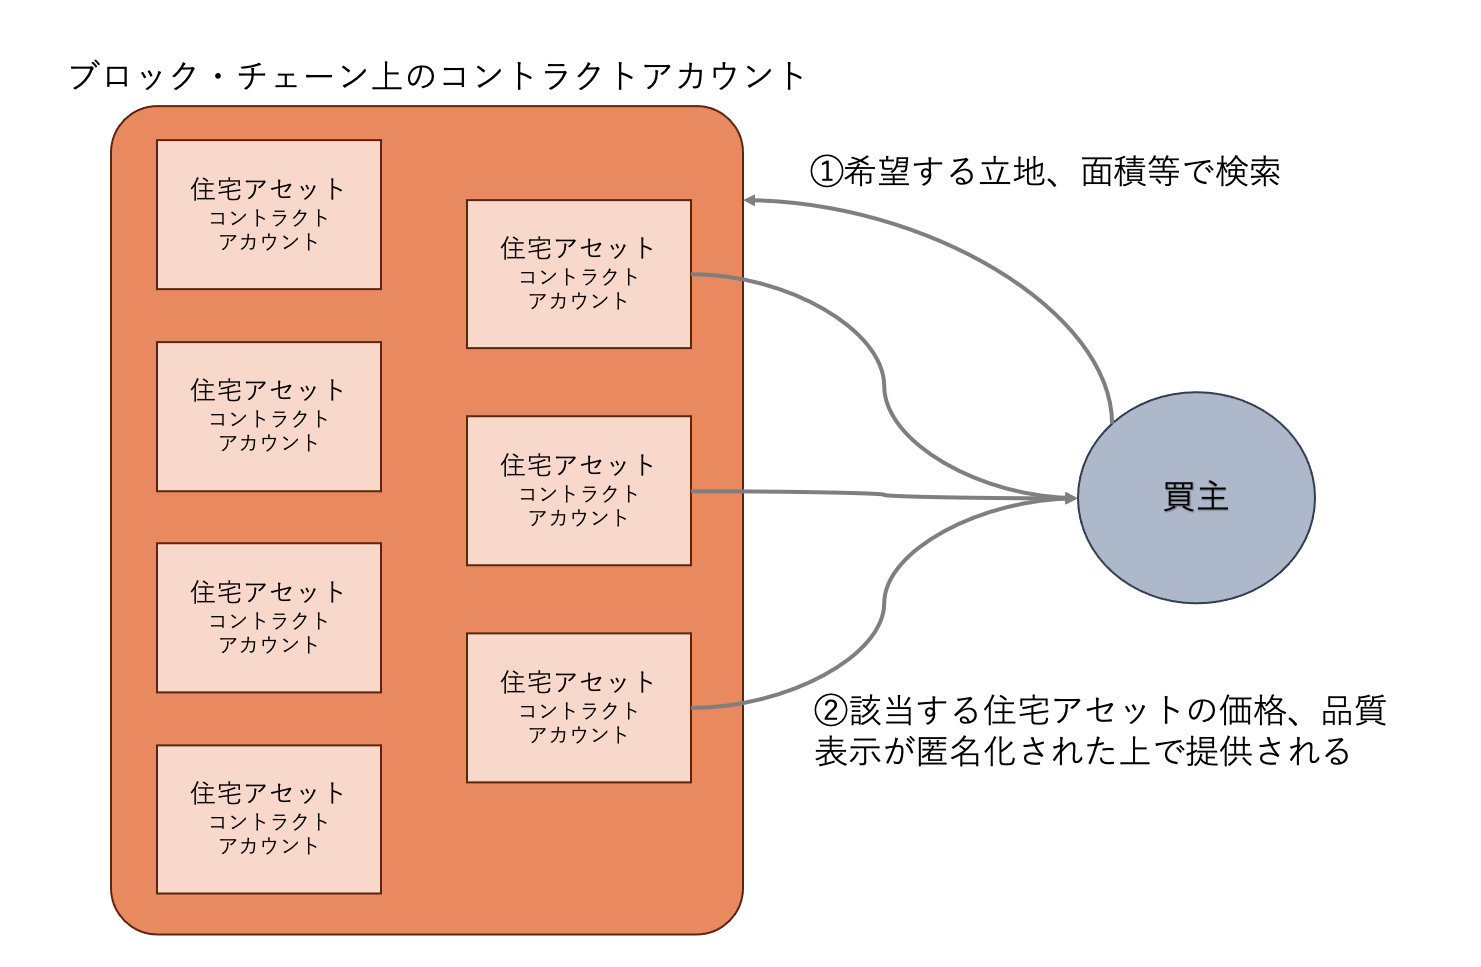
\includegraphics[width=11cm]{search.png}
 \caption{ブロックチェーン上の住宅アセットの情報探索}
 \label{search}
\end{figure}

\begin{figure}
 \centering
 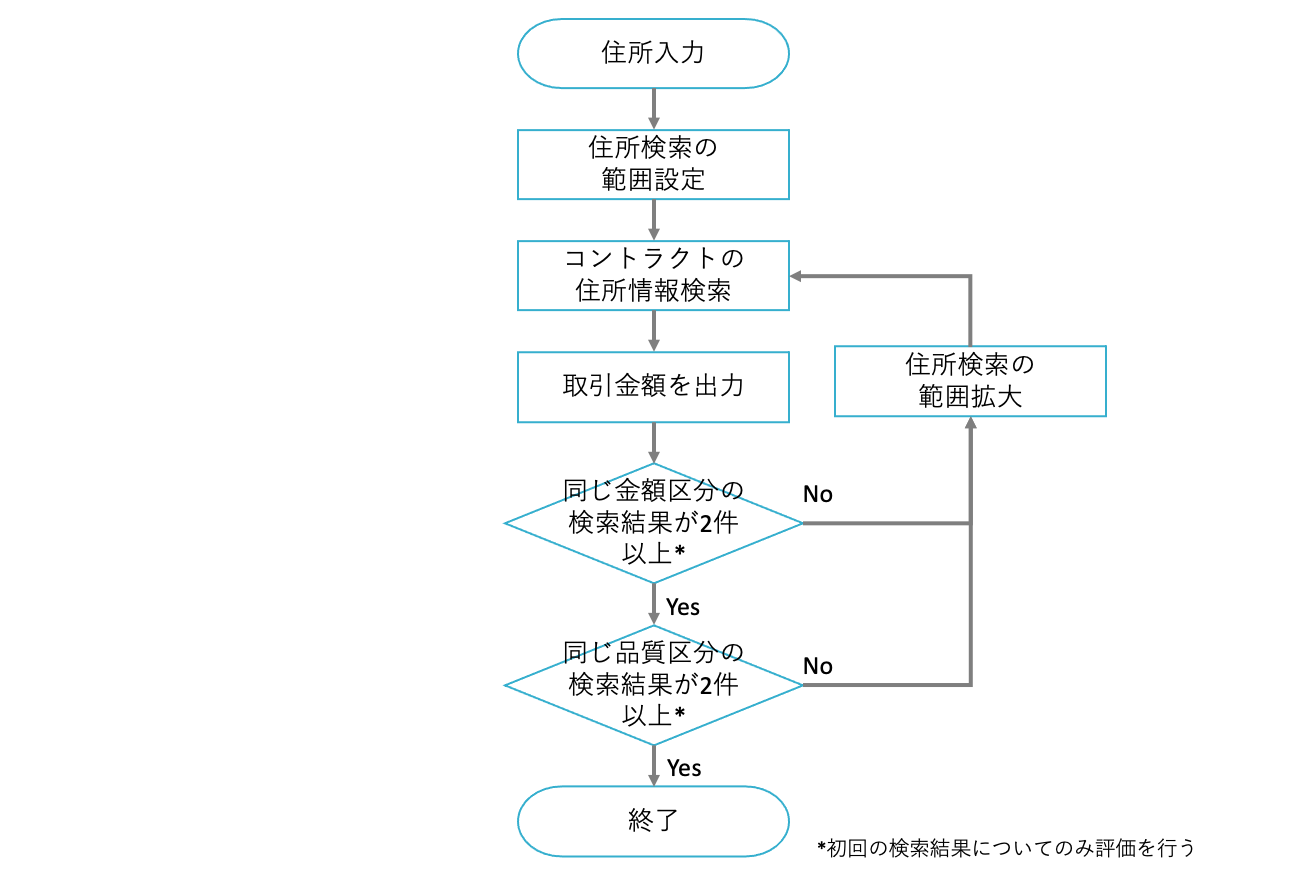
\includegraphics[width=12cm]{searchflow.png}
 \caption{取引情報の検索処理}
 \label{flow}
\end{figure}

\section{保険契約}
保険契約のコントラクトアカウントは、住宅の所有期間に渡って、売主を被保険者として存在している。住宅取引にあたっては住宅品質の再評価と、再評価された品質に基づく新たな保険契約の締結が必要となる。この新たな保険契約の締結は、売主または買主からのトランザクションで開始される。保険契約コントラクトはインスペクターに保険契約の対象となる住宅アセットの品質を調査し、住宅性能表示を行う指示を出す。インスペクターは対象住宅の住宅状況評価を行い、住宅アセットの住宅性能表示を更新する。次に、保険契約コントラクトは保険会社に住宅性能表示の検証の指示を出す。住宅性能表示の情報は保険料算定の前提となるため、保険会社には住宅性能表示が正しく実施されているか検証するインセンティブが発生する。インスペクターによる住宅性能表示の更新と保険会社による検証が終了すると、住宅アセットは住宅性能表示の情報を保険契約コントラクトに送信し、保険契約コントラクトはその情報に基づいて保険料を算出し、保険契約を締結する。保険契約の被保険者(保険金受取人)は住宅の所有者であり、住宅取引によって所有者が売主から買主に変わると被保険者も買主に変わる(図\ref{insurance})。
%現行の住宅瑕疵担保責任保険では、保険料は売主が負担することが一般的だが、本研究で検討する保険契約では、売主、買主のどちらが保険料を負担する形も設計可能である。

\begin{figure}
 \centering
 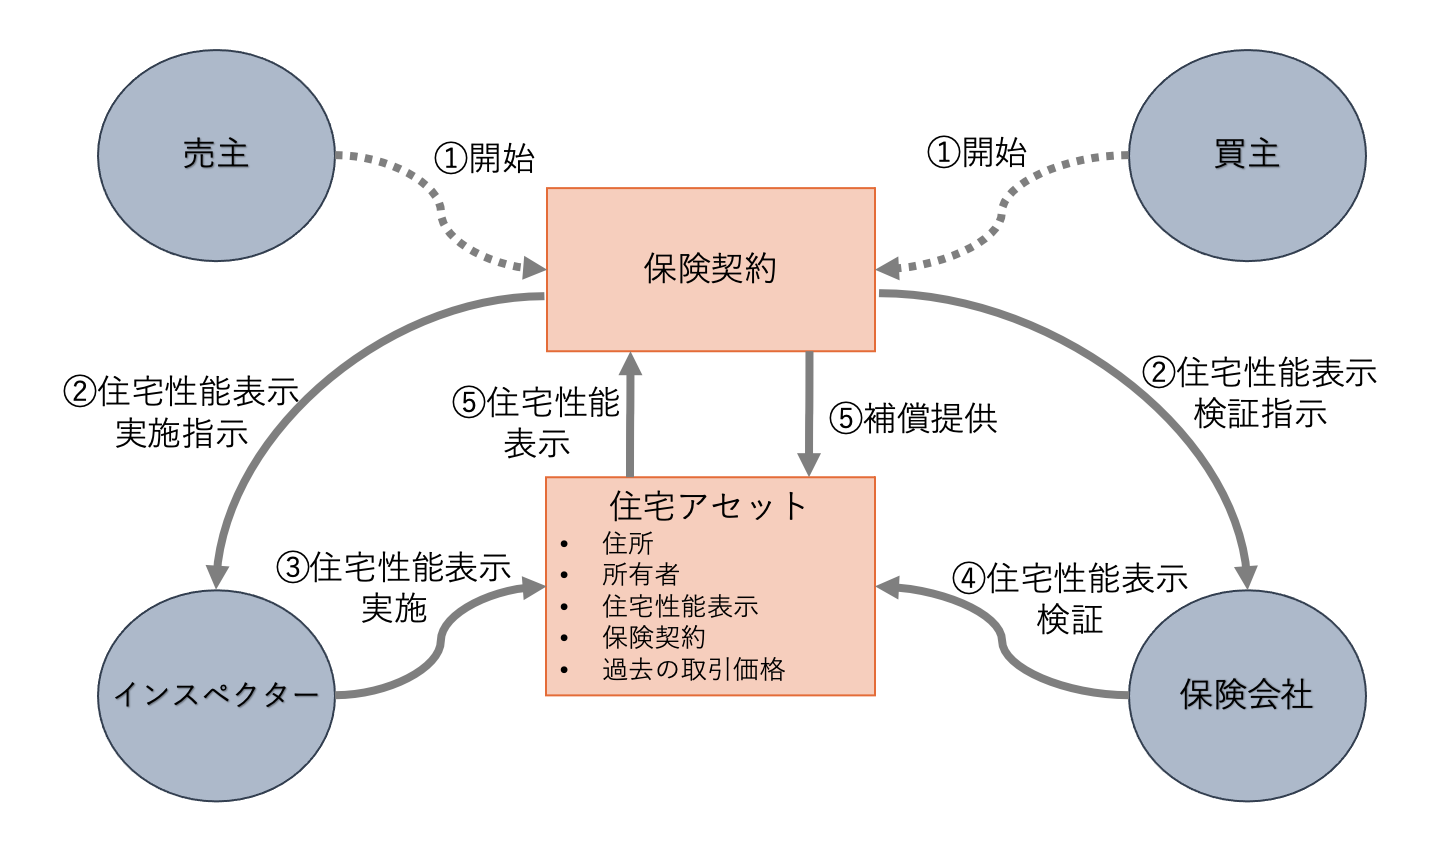
\includegraphics[width=12cm]{insurance.png}
 \caption{保険契約の締結}
 \label{insurance}
\end{figure}

\section{住宅取引契約}
住宅取引契約のコントラクトアカウントは、売主または買主からのトランザクションで開始される。売主は住宅アセットの所有者変更のトランザクションを住宅取引契約コントラクトに送信し、買主は取引代金のデジタル通貨送金のトランザクションを送信する。住宅取引契約コントラクトは売主と買主のトランザクションが揃った場合に、住宅アセットの所有者情報の変更を行い、同時に売主にデジタル通貨を送金する。これにより住宅アセットコントラクトに登録される所有者が買主に変更される。住宅取引契約アカウントは、所有者の変更と同時に住宅アセットの取引価格の情報も更新する。住宅アセットは、保険契約のコントラクトに対して所有者情報を変更したメッセージを送り、保険契約の被保険者を変更させる。(図\ref{spa})。

\begin{figure}
 \centering
 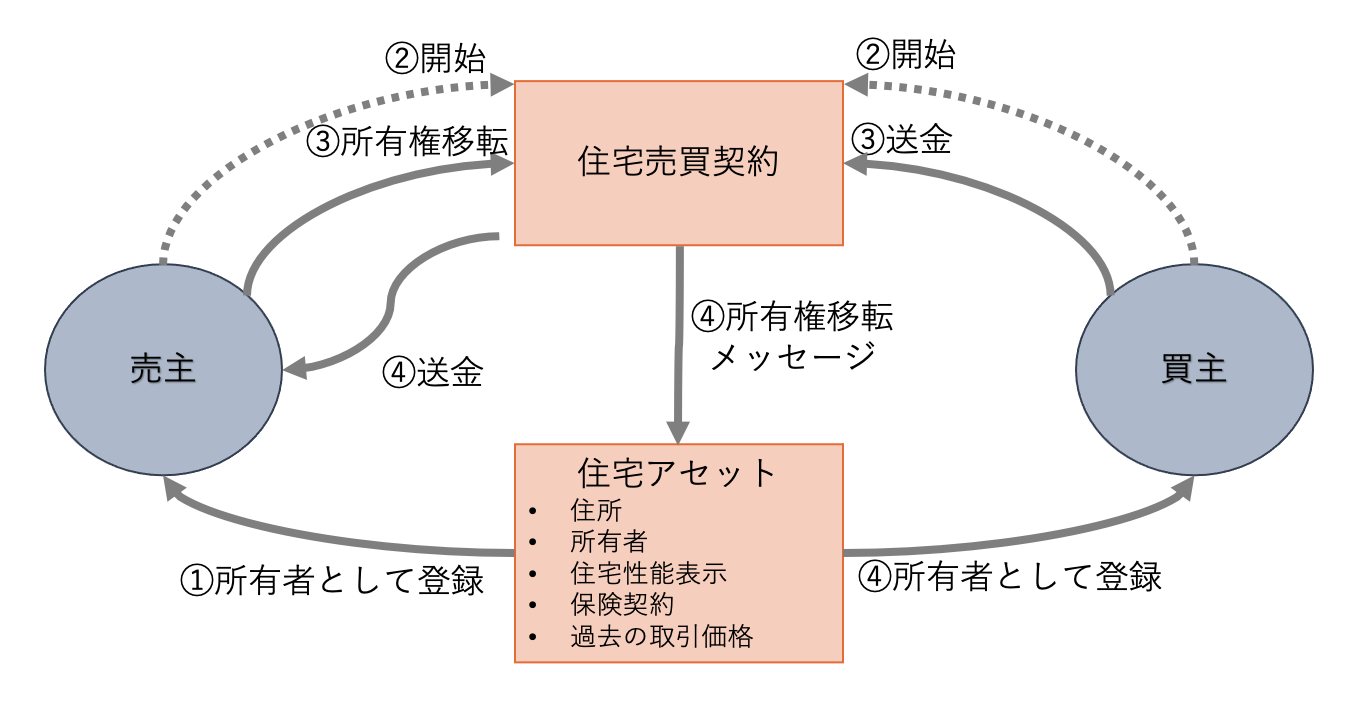
\includegraphics[width=11cm]{spa.png}
 \caption{住宅売買取引}
 \label{spa}
\end{figure}

\section{問題解消への貢献}
住宅アセット、保険契約、住宅取引契約のコントラクトの組み合わせにより、買主は購入する住宅の品質を把握し、購入後に住宅の品質が予想外に低かった場合に発生する修繕費用などの損失を回避できる。これによって中古住宅市場における情報の非対称性の問題を解消することができる。売主にとっては、保有期間中に行ったメンテナンスやリフォームが住宅性能表示を通して取引価格に影響するため、適切なメンテナンスを行うインセンティブが発生する。これにより、高い品質の住宅供給の増加が期待できる。住宅の価格、品質の情報は住宅取引契約から住宅アセットに直接更新され、修正や改ざんはできない。売主と買主は、住宅アセットの取引情報の検索を通して住宅の価格水準を把握し、値決めを行うことができる。

\chapter{検証}
情報の非対称性の解消が住宅取引に与える影響を検証するため、マルチエージェントシミュレーションを行った\footnote{シミュレーションに用いたコードは付録に記載する。}。マルチエージェントシミュレーションは、複数の自律的なエージェントからなるシミュレーションである。本研究では、売主と買主をエージェントとし、住宅取引を単純化したゲームでエージェント間の影響を検証した。

\section{ゲームのルール}
現在の住宅取引は、売主と買主の間で住宅の品質に関する情報の有無が異なるため、非対称情報ゲームとして記述することができる。売主は所有する住宅の品質を知っており、品質に比べて不当に高い値付けを行うか、品質に応じた値付けを行うかの2つの選択肢をとり得るものとする。売主は住宅の保有コストを負担しており、住宅の売却ができなかった場合、保有コスト分の損失を被る。売主と買主が出会う率が十分に高く、流動性ディスカウントが無視できる場合に、住環境を得るための保有コスト$v_s$は$v_s=r_sP_s$となる。ここで、$r_s$は売主の割引率、$P_s$は売主の提示価格である。買主は売主からの価格の提示を受けて買うか買わないか判断し、購入した後で住宅の品質に応じて利得を確定する。住宅の品質に基づく、買主にとって妥当な価格を$P_b$、住宅保有コストを$v_b=r_bP_b$(ただし、$r_b$は買主の割引率)とする。ここで、$P_b$は売主にとっても住宅の品質に基づく中立的な価格であり、$P_s=P_b$の時の場合、売主には住宅取引による利得は発生しないものとする。以上に基づく売主と買主の各戦略における利得は表\ref{ritoku}となる。

\begin{table}
\begin{center}
\caption{売主・買主の利得}
\label{ritoku}
\begin{tabular}{l|cc}
売主\買主 & 買う & 買わない \\ \hline
高い値付け($P_s>P_b$)   &  $P_s-P_b$,  $P_b-P_s$ &  $-v_s$,  $-v_b$  \\
妥当な値付け($P_s=P_b$)   &  0, 0 &  $-v_s$,  $-v_b$ 
\end{tabular}
\end{center}
\end{table}%

\section{売主、買主のクラス}
売主のクラスは、ゲームが終わるごとにランダムに選んだ他の売主と自身の得点を比較し、次のゲームでの戦略を決める。売主エージェント$i$がランダムに選んだ隣人エージェント$j$の戦略を真似する確率を以下の定義とし、隣人の利得が高いほど真似する確率が高くなるものとした(Tanimoto et al 2012)\cite{tanimoto2012}。ここで、$\Pi_i$、$\Pi_j$はエージェント$i$、$j$の利得であり、温度計数$\kappa$は0.1とした。戦略の更新は、全てのエージェントが一斉に戦略更新するシンクロ更新を用いた。

\begin{equation}
P_{i \gets j}=\dfrac{1}{1+\exp\biggl(\dfrac{\Pi_i-\Pi_j}{\kappa}\biggr)}
\end{equation}

買主のクラスも売主と同様に、ゲームが終了するごとにランダムに選んだ他の買主と自身の得点を比較し、次のゲームでの戦略を決めるものとし、戦略変更の確率も売主と同様とした。住宅取引では、売主は住宅の売却後には買主として、買主は住宅の購入後には売主として市場に参加することになるが、本研究のシミュレーションでは、売主は繰り返し売主として、買主は繰り返し買主としてゲームに参加するものとした。

\section{シミュレーションのクラス}
シミュレーションにあたって、売主、買主のネットワークはBarab\'{a}shi-Albert Scale Free Network(BA-SFネットワーク)を用いた。BA-SFネットワークは、エージェント間のネットワークが繋がる際に次数の高いエージェントの方がネットワークを獲得しやすいというモデルであり(増田,今野 2010)\cite{masuda2010}、SNSなど見られるような、影響力のあるエージェント(インフルエンサー)が、ゲームが進むにしたがって影響力を増していく様を再現することができる。ゲームの参加者は売主、買主それぞれ2,000人とし、平均次数$k=4$とした。

\chapter{評価}


\chapter{関連研究}
不動産分野におけるスマートコントラクトの活用に関する論文は多くない。Karamitsos et al(2019)\cite{karamitsos2019}は、住宅の賃貸借契約を締結し、賃料の支払いを行い、賃貸借契約終了時の敷金の精算を行うイーサリアムブロックチェーンを利用したスマートコントラクトの設計を行なっている。スマートコントラクトの概略や設計の思想に重きが置かれており、現実の不動産分野での利用に向けた課題についてはほとんど触れられていない。
不動産分野、住宅分野でのスマートコントラクトの活用には、その対象が実物資産であることから、不動産、住宅の資産としての特性、取引市場の市場としての特性についてより詳細な検討が必要である。

Mashatan and Roberts(2017)\cite{mashatan2017}は、カナダの不動産市場を対象として、取引コスト、取引時間を改善するため、ブロックチェーン技術を活用した入札、台帳システムを提案している。カナダにおける不動産の取引コストが、取引価格の11〜22\%と非常に高いこと、無権利者による詐欺が発生していることなどが研究の背景にある。また、日本と同様、不動産仲介業者が一つの不動産取引で売主と買主の双方の代理人に同時に就く、いわゆる「両手取引」がカナダでも行われており、仲介業者が入札を通して取引価格を最大にするよりも、ある程度のところで売主と買主を妥協させて取引を成立させ、確実に手数料を獲得しようとすることも問題視している。仲介業者が誠実に入札を行わないことで、本来獲得可能な利益が獲得できないという不利益が、売主に生じる。仲介業者の不誠実な入札が発生する原因は、入札手続きが売主、買主双方にとって不透明なためであると分析し、この問題を解消するため、ブロックチェーンを利用し透明性を確保した入札システムを提案している。また、不動産取引は売主、買主、仲介業者だけでなく、銀行や弁護士など幅広い関与者があることで取引に時間がかかり、取引の進み具合も他の参加者からは把握し難いことを問題視し、ブロックチェーン上の台帳の利用により取引の可視化と取引時間の短縮が可能であると指摘している。
ブロックチェーンを用いて市場の透明性と情報の正確性を向上しようという動機は本研究と共通するものである。また、不動産市場の持つ問題から出発しており、現実的な問題への対応として評価できる。一方で、実物資産である不動産の情報をどのようにブロックチェーンに取り込むかについては言及されていない。不動産の不正確な情報がブロックチェーン上で共有されることは、参加者の混乱を招くとともに、システム全体の信頼を損ねる。

%斉藤(2017)\cite{saito2017}も、不動産取引が売主、買主などの取引関係者が一同に会して行われている背景として、「意思確認の効率化と、契約不履行による様々なリスクを避けるためといった理由があると考えられる」と指摘した上で、意思確認とリスク回避の手段としてスマートコントラクトを用いて売買を成立させることができるモデルを紹介している。

ブロックチェーン、スマートコントラクトの、実際の取引への導入を検討するにあたっては、実務を踏まえた検討が求められる。本研究の特徴は、スマートコントラクトによって実物資産を取引する際に課題となっていた、資産をどのようにデジタルに表現するかの問題について、現実に存在する制度を活用して解決可能な方法を提示したことにある。


\chapter{結論}
\section{本研究の結論}
本研究では日本の中古住宅の取引におけるスマートコントラクトの活用が、中古住宅の価格や品質の情報を利用可能にする事によって、取引価格の向上に資することを検証した。日本の家計における住宅資産は、土地の価値も含めると、現金・預金等に匹敵する規模があり、その市場価値が減少した場合には家計の投資や消費にマイナスの影響を与える可能性が高い。これまで日本の中古住宅市場は、売主と買主の間で住宅の品質や価格についての情報の非対称性が大きく、レモンの市場となっていた事から活性化していなかった。本研究の検証により、スマートコントラクトでの住宅取引を行い、価格や品質の情報をブロックチェーン上に公開することは、中古住宅取引の活性化に繋がり、中古住宅の取引価格を引き上げると考えられる。スマートコントラクトは、参加者の利便性と情報の信頼性を同時に満たすことのできるアプローチであるが、その活用にあたっては個人情報の取り扱いに配慮する必要がある。加えて、住宅という実物資産をスマートコントラクトの対象とする場合、住宅の品質情報などを正確にスマートコントラクト上に取り込む仕組みが重要となる。日本では建物状況調査などの取り組みが政策として推進されていたが、活用が進んでいなかった。これらの仕組みがスマートコントラクトに取り込まれる事によって、信頼性のある資産の情報が全ての参加者に利用可能となる。

\section{未解決の問題}
\subsection{不動産登記との連携}
不動産登記は、一つ一つの土地、建物などについて、どこに所在し、誰が所有しているかを記録したものであり、法務省が管理している。不動産登記制度が現状のまま存続する限り、スマートコントラクトによる所有者の変更と、不動産登記上の所有者の変更をどのように連携させるかが課題となる。中島(2019)\cite{nakajima2019}は、不動産登記のブロックチェーン化を進めるにあたっては、法務省自身が主体とならなければならないと指摘している。

\subsection{スマートコントラクトの費用}
本研究で検討したイーサリアムブロックチェーンを基盤とするスマートコントラクトの実装にあたっては、必要なガスの総量と単価の設定について検討する必要がある。必要なガスの総量は、トランザクションとスマートコントラクトの処理に要する計算のステップから算出可能だが、ガス単価の相場は需給バランスによって変動する\footnote{2021年1月2日時点の平均ガス単価は60gwei(gweiはEtherの単位で、$10^{-9}$Ether)であり、0.92ドル程度。https://etherscan.io/gastracker}。そのため、ガス単価の上昇によりスマートコントラクトの費用が増加した場合、スマートコントラクトが利用されない可能性がある。現在の住宅取引において売主と買主は、不動産仲介会社を利用した場合には、住宅価格の3\%程度の手数料をそれぞれ負担しており、2000万円の住宅の取引では仲介手数料は60万円程度になる。スマートコントラクトが広く利用されるためには、その費用が仲介手数料の水準よりも低くなり、売主及び買主の短期的な利益となることが必要であると考える。この点の検証には、必要なガスの総量の検証とガス単価相場の動向の分析が必要である。

\subsection{住宅ローンの影響}
金融機関は住宅ローンを通して住宅取引に影響を与えている。買主は、住宅購入資金を全額自己資金で賄うことは稀であり、住宅ローンを利用することが一般的である。そのため、買主が品質情報や過去の取引情報から住宅の売出し価格が妥当だと判断しても、金融機関の担保評価が低ければ住宅ローンの融資額が低くなり取引が成立しない。そのため、中古住宅の取引価格が上昇するためには、金融機関の担保評価が上昇することが欠かせない。金融機関の担保評価は、債務不履行が発生した場合に、担保の住宅を売却して回収できる金額を想定して算出される。中古住宅の品質情報や取引価格の情報が参照可能となる事は、金融機関の担保評価においても、プラスに働くと考えられる。

\subsection{住宅の個別性}
売主と買主の行動に注目し住宅の品質のクラスは単純化した。現実の中古住宅市場は、住宅ごとの個別性が高く、住宅が所在する立地も異なる事から、一つとして同じ住宅はない。スマートコントラクトが中古住宅市場に与える影響を検討するためには、このような住宅の個別性を踏まえた検証が必要であると考えられる。


\bibliographystyle{jplain}
\bibliography{export}

\appendix
%\def\thechapter{Appendix\Alph{chapter}}
\chapter{マルチエージェントシミュレーションのコード}
\footnote{本研究のシミュレーションのコードはhttps://github.com/keyskey/SPDpyを参考に作成した。}
\section{Sellers Class}
\section{Buyers Class}
\section{Simulation Class}


\end{document}
